\chapter{Etat de l'art : Analyse, etude et outils}
\label{sec:Etat de l'art}

\section{Etude avant réalisation}


\subsection{Analyse du marché des applications mobiles}
Avant de commencer la réalisation de l'application, j'ai étudié le marché actuel en termes de développement mobile et j'ai choisi la meilleure solution possible avec la problématique suivante : réaliser seul une application disponible à la fois sous Android et sous iOS. A l’heure actuelle, il existe plusieurs options pour développer une application mobile :

\begin{itemize}
    \item Un développement natif, codées dans un langage donné avec un code source pour chaque plateforme (Objective-C ou Swift pour iOS, Java ou kotlin pour Android) .
    
    \item  Une solution cross plateforme : Les solutions telles que Xamarin(Microsoft), React Native (Facebook) ou Flutter (Google) permettent de construire des applications iOS et Android avec du code commun à chaque plateforme.  
    
    \item Une solution hybride : Les technologies de type Gordova permettent en utilisant des technologies web de développer des applications qui embarqué une WebView.

\end{itemize}

Il existe aussi le terme web app qui désigne un site web qui s'adapte parfaitement aux appareils mobiles. Ces sites ne peuvent pas tirer parti des spécificités des smartphones comme accéder au carnet de contacts par exemple. Pour la réalisation de l'application, au sein de mon stage, cela ne correspond pas aux attentes du client et cette solution est éliminée d'office.

Le terme d’application native n’est pas très connu du grand public, cela représente pourtant la grande majorité des applications que nous téléchargeons chaque jour. Finalement, quand on pense aux applications mobiles, on pense inconsciemment aux applications natives. Mais alors, qu’est-ce qu’une application native ? C’est une application qui est développée spécifiquement pour un système d’exploitation. Un logiciel disponible sous Ubuntu par exemple fonctionnerait pas sur Windows et vice-versa. Cela signifie que le langage de programmation permettant de déveloper une application est différent d’un système d’exploitation à un autre. Par exemple, iOS utilise majoritairement le langage Objective-C, tandis qu’Android utilise Java. Chacun a ses spécificités. C’est pourquoi les développeurs précisent sur quelle plateforme ils développent. Un développeur Android ne sait pas forcément développer sur iOS et vice-versa.

Les applications hybrides sont des applications crées avec des technologies web (HTML, CSS et JavaScript) et qui sont exécutées dans une application native à travers une WebView. Pour simplifier, il s'agit d'un navigateur web dont la barre d’adresse est masquée, c'est une encapsulation d'un site web classique. Cependant, elle s’appuie également sur des technologies natives mobiles via des bridges pour pouvoir utiliser certaines fonctionnalités d'un smartphone. Bien que développée avec des technologies web, il s’agit d’une véritable « application » dans le sens où elle sera téléchargée depuis les magasins d’applications. Par exemple, l'application LinkedIn est une application mobile hybride. Il est donc possible de publier une application hybride sur un store et l’installer comme une application native contrairement à la web app qui n’est consultable seulement depuis un navigateur.


Depuis 2015, un nouveau concept a vu le jour, il s’agit d’un mélange entre les applications hybrides et les applications natives. Appélé simplement Framework, les plus connus sont React Native (créé par Facebook), NativeScript (créé par Telerik et soutenu par Google) et Xamarin (rachetée par Microsoft en 2016) . Le concept est simple : proposer le meilleur du natif et le meilleur de l’hybride, en alliant performances et comportements natifs. Dans les deux cas, le code source est écrit en JavaScript via React (pour React Native) ou Angular (recommandé pour NativeScript). La différence majeure avec les applications hybrides est que ce nouveau concept ne s’appuie plus sur les WebView. Les composants écrits en JavaScript sont transformés en composants natifs. Les deux architectures des Framework se basent sur un bridge asynchrone entre le code JavaScript et les couches UI natives pour piloter les composants. React Native (RN) utilise JavaScriptCore sur iOS et sur Android, NativeScript utilise V8 sur Android et JavaScriptCore sur iOS.  Les éléments utilisés auront une apparence différente en fonction de la plateforme sans avoir besoin de spécifier la platform. L’utilisateur retrouvera les composants qu’il a l’habitude de voir et qui garderont le même comportement habituel sur son OS mobile, ce qui est important en termes d’expérience utilisateur (UX) car elles seront conformes aux normes imposées par le système d'exploitation.



\subsection{Diagnostic et proposition de solutions }

Pourquoi la plupart des applications sont-elles natives ? La raison est que les applications natives ont un certain nombre d’avantages significatifs par rapport aux alternatives. 
Les applications natives offrent aux utilisateurs, l’expérience la plus rapide, la plus fiable et la plus réactive. Les applications natives rendent aussi l'accès aux fonctionnalités d'un smartphone plus facile comme l’accès à la caméra, le microphone, l’accéléromètre et autres. Une application native ne permet pas seulement d’avoir des performances accrues et d’accéder simplement à toutes les fonctionnalités du téléphone. Lorsqu’elles sont bien pensées et réalisées, elles respectent les codes design de chaque plateforme. Il existe des centaines de différences entre le système d’exploitation de Google et celui d’Apple. Les applications natives permettent de s’adapter à chaque plateforme afin de proposer aux utilisateurs une expérience optimale et pleinement compatible avec la plateforme correspondante. L'inconvénient majeur est que ce code écrit pour l'une des plateformes sera complétement inutilisable sur l’autre plateforme et vice versa, il faut donc travailler avec différentes bases de code pour chaque plateforme. Les applications natives coûtent généralement plus cher à réaliser que les autres applications, web ou hybrides. Essentiellement pour des questions de compétences, performances et de temps. La plupart des développeurs se spécialisent généralement dans l’une des deux plateformes. La création d’une application sur les deux plateformes nécessitera donc deux développeurs (ou équipes), ce qui ajoute du temps et une plus grande complexité pour maintenir à jour les deux applications.



Tous les avantages des applications hybrides découlent du fait qu’au lieu de créer deux applications, une seule application est construite. Cela représente une énorme économie en termes de temps et un maintien plus simple de l’application. Les applications hybrides sont aussi plus faciles à adapter à chaque plateforme puisqu'il s'agit d'un site web encapsuler dans une application classique. Une fois que l’application est construite pour une plateforme, généralement de faibles modifications sont nécessaires pour avoir une application parfaitement compatible avec les autres plateformes et garantir un accès aux fonctionnalités de l’appareil. Une solution hybride garantie une application 100 \% compatible multiplateforme. 
Enfin, en tenant compte du fait que les utilisateurs d’Apple iOS et de Google Android ont tendance à être très fidèles à leurs plateformes, et parce qu’ils les utilisent depuis des années, ils sont habitués à la façon dont les choses fonctionnent dans les applications natives et il s’agit d'un vrai problème pour les applications hybrides puisque le design de l’application sera le même peu importe la plateforme. En effet il existe aujourd’hui des différences de design notable entre Android et iOS. Google met régulièrement en avant le matérial design lors de ses conférences I/O notamment en 2018 où la version 2 du material design a été introduit comme un principe pour développer des applications agréables sur son système d’exploitation mobile. Ses principes sont naturels pour les utilisateurs puisqu’aujourd’hui un grand nombre de personne sont fortement attachés aux services du géant et utilise ses applications qui respecte à la lettre ces principes notamment via Gmail ou Google Maps. De son côté Apple est le premier à avoir introduit des lignes directrices d'interface humaine pour son OS mobile. Le Flat design exclut tout effet de profondeur, d'ombre portée, de reflets pour se concentrer sur l'essentiel et trouver le plus court chemin pour transmettre une information. Selon la liste officielle des raisons communes de rejet d’applications sur l’App Store, « Apple accorde une grande importance aux interfaces propres, raffinées et conviviales. Assurez-vous que votre interface utilisateur répond à ces exigences en planifiant votre conception avec soin et en suivant nos guides de conception et UI Design Dos et à ne pas faire »\cite{AppleRejection}. C'est un des principaux inconvénients que l’on n’arrive pas à égaler le native feeling (“sentiment” d’application native). En effet, le fait de devoir passer par une WebView créé une couche intermédiaire entre le téléphone et la manipulation de l’utilisateur. Il y a donc une certaine latence entre le temps où l’utilisateur touche le téléphone et le moment où l’application réagit. Cette sensation se traduit par un problème de performance, il s'agit d'un inconvénient majeur. Il y aura toujours un fossé entre un navigateur web de bureau et un navigateur web de téléphone. La WebView ne donne pas accès à toute la puissance de calcul dont dispose le téléphone, et les animations en pâtissent fortement. De plus puisqu'il s'agit d'un site web, chaque clique donne lieu à un chargement de page plus ou moins long en fonction de la connexion du smartphone.




Concernant les solutions cross-platform, j'ai choisi de sélectionner pour mon étude, le Framework React Native pour diverses raisons : Sa communauté est très active, Sa notoriété est grandissante et surtout il s'agit d'un Framework Open Source crée par l'entreprise Facebook. Avant la création de React Native, Facebook à crée React js qui cible les interfaces web et aujourd’hui est très utilisée. Suivant cette logique, Facebook à lancé en 2015 React Native qui est un moteur de rendu d’applications natives et repose sur la même API que React. Il existe quand même un certain nombre de différences significatives entre React js et React Native que je ne développerai pas.  Comme tous les Frameworks multiplateformes, React Native permet de développer une base de code commune aux différentes plateformes qui sera déployée simultanément sur les stores Android et iOS. Cette force des solutions cross-platform offre un gain de temps considérable par rapport à du développement spécifique, tout en étant aussi performant. Un seul code à développer signifie un seul code à faire évoluer. Un seul développeur est donc capable de maintenir l’application et d’y ajouter de nouvelles fonctionnalités. Il n’aura en plus pas besoin de maîtriser des langages spécifiques au mobile, puisque React Native est un Framework JavaScript, le langage de développement le plus répandu et par conséquence dispose d'une communauté énorme. React Native permet également de créer une expérience utilisateur cohérente en utilisant des outils de développements cohérents basés sur javascript et la librairie React. En effet, le principe essentiel de React Native est le développement via des composants, chaque composant est écrit en JavaScript puis à l’aide d’un bridge ce code va être converti en composant natif. Il s'agit des mêmes composants que ceux des applications natives plutôt que d’utiliser des WebViews comme le font d’autres Framework multiplateformes (Cordova par exemple).

\begin{figure}[htp]
  \centering
  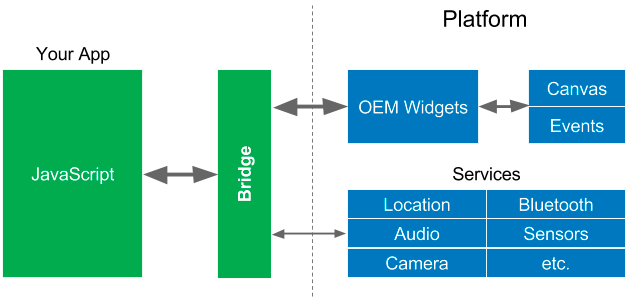
\includegraphics[width=7cm]{images/reactnative}
  \caption{Fonctionnement de React Native.}
  \label{fig:fonctionnement-rn}
\end{figure}

L’utilisation de composant natif permet des performances pratiquement identiques à celles des applications développées en code natif et évidement aucun chargement superflu est nécessaire. Une application écrite en React-Native ne dépend pas de la connexion internet de l’utilisateur, le code écrit avec React Natif est interprété en composant natif comme expliqué précédemment, il est donc possible de développer une application offline et donc limite les connections superflues contrairement aux applications hybrides qui sont totalement dépendantes de la qualité du réseau.  Cette interprétation en composant natif permet à un utilisateur iOS ou Android de retrouver un design cohérent entre l’application et le reste de son OS ou de ses autres applications téléchargées, il ne sera pas perdu en naviguant dans l’application, puisqu’il retrouvera l’ergonomie à laquelle il est habitué.
Contrairement aux applications hybrides, il ne s’agit pas d’une solution compatible à cent pourçent entre les différentes plateformes. Malgré cela, il est possible d'ajouter du code spécifique aux différentes plateformes en cas de besoin spécifique. Par exemple, l’application Instagram partage 85 \%  de code commun entre Android et iOS, le reste du code est spécifique à chaque plateforme. Heureusement, lors du développement React Native propose de compiler en fonction de la plateforme cible permettant de tester rapidement la compatibilité de l'application et d'avoir un code entièrement compatible et partagé entre Android et iOS. Facebook n’est pas seul pour mettre à jour son Framework, puisque plus de la moitié des nouvelles contributions sont ajoutées en Open Source par la communauté. Cette proportion particulièrement élevée indique une communauté particulièrement active. Les mises à jour sont donc plus fréquentes, et les réponses beaucoup plus rapides lorsqu’un développeur se retrouve bloqué sur une fonctionnalité de son projet.Cette communauté met au point de  très nombreuses librairies telles que Native Base ou React Native Element qu'il est possible d'ajouter rapidement à un projet existant pour étendre les composants disponibles de base.

 

Développé par Facebook depuis début 2015 et bénéficiant d’une large communauté, React Native continue d’évoluer avec le soutien de nombreux contributeurs sur Github. React Native est une technologie très prometteuse avec un énorme potentiel, qui a déjà été dûment appréciée par des géants comme Airbnb, Baidu, Discovery, Instagram et d’autres. Constamment améliorée et mise à jour par ses fondateurs, je pense qu'il s'agit d'une alternative à part entière à Objective C, Swift et Java.
 

\begin{figure}[htp]
  \centering
  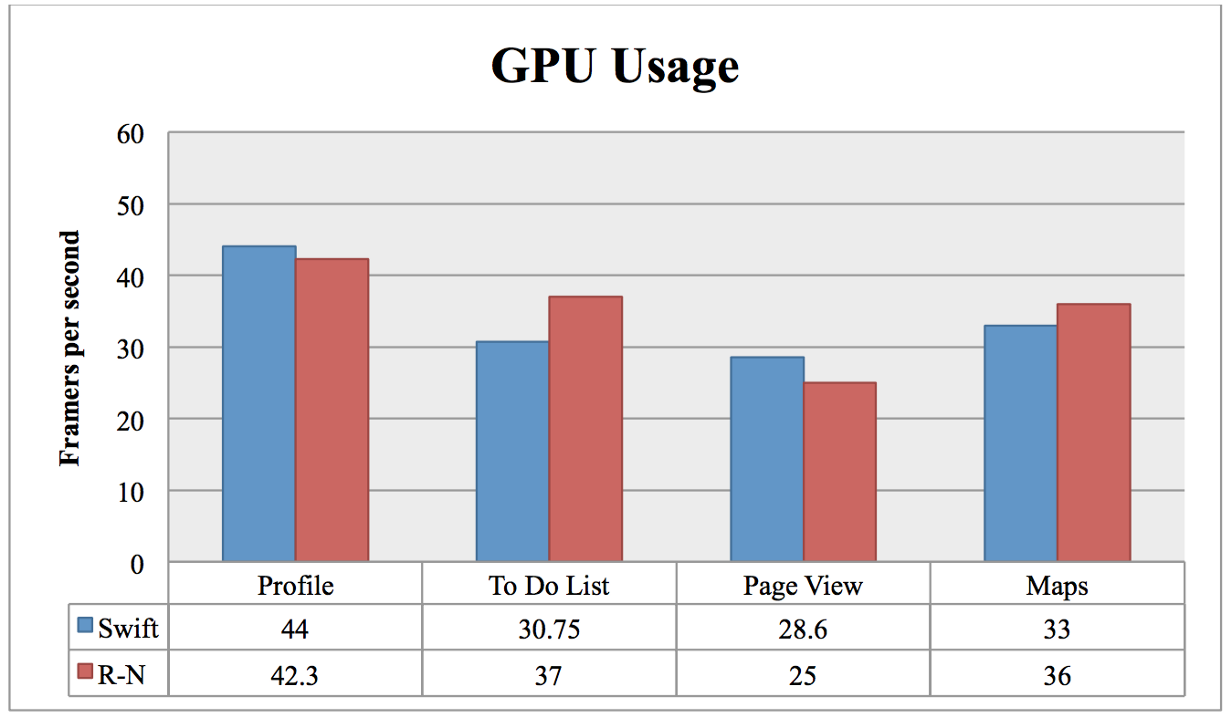
\includegraphics[width=7cm]{images/GPUusage}
  \caption{Différence de performance entre React Native et swift.}
  \label{fig:performance}
\end{figure}

En résumé, j'ai choisi de développer l'application mobile pour le système de recommandation d'articles en React Native. À la vue des contraintes de temps, de réactivité, d'évolutivité et du maintien de l’application. Pour moi il s'agit d'un bon compromis entre les applications natives et les applications composé uniquement de WebView.  


\section{Environnement de travail}

Dès le début de mon stage, le LRI m'as prêté un ordinateur portable sous Windows 10 pour travailler. De plus, j’ai mon téléphone personnel, un iPhone pour tester mon application mobile tout au long du développement, J’ai adapté mes choix logiciels en fonction de mes besoins pour ce stage.  

\subsection{IDE}

Visual Studio Code est un éditeur de code source développé par Microsoft pour Windows, Linux et OS X. Il est gratuit, open-source et inclut la prise en charge du débogage ainsi que le contrôle Git embarquer. Les fonctionnalités que Visual Studio Code contient sont prêtes à l'emploi mais il est possible d'ajouter des extensions en fonctions de ses besoins via un marketplace. Les extensions VS Code permettent d'ajouter la prise en charge des langages, des débogueurs. Pour mon travail sur React-Native,  j'ai installé comme première extension React Native Tools. Cette extension permet d'ajouter un environnement de développement spécifique à React Native. En utilisant cette extension, il est possible de lancer les commandes React-Native depuis la palette de commande VS Code et ajoute l’auto-complétions pour les APIs de React Native. Une seconde extension nommée Setup ESLint qui est un outil permettant d’améliorer la qualité du code JavaScript. Ce langage étant très permissif, il est très simple de glisser facilement sur du code illisible par un autre collaborateur. Eslint permet de structurer le code de façon uniforme. Tous les développeurs devront alors suivre les règles, le code est ainsi plus lisible. Dans le cas d'un développeur isolé comme durant mon stage, EsLint m’aide beaucoup à maintenir un code propre et uniforme.

\subsection{Gestion de version}

Un gestionnaire de version est un système qui enregistre l'évolution d'un fichier ou d'un ensemble de fichiers au cours du temps de manière à ce que l’on puisse rappeler une version antérieure d'un fichier à tout moment. Pour le développement de mon application, j'ai choisi d'utiliser Github. Github, c’est quoi ? Le nom GitHub est composé du mot « git » faisant référence au système de contrôle de version open-source et le mot « hub » faisant référence au réseau social bâti autour du système Git. Comme son nom ne l’indique pas, Github est un logiciel de gestion de version, mais pas que. C’est aussi un outil de développement collaboratif. GitHub est centré vers l'aspect social du développement. C’est le plus grand espace de stockage de travaux collaboratifs au monde. En plus d'offrir l'hébergement de projets avec Git, le site offre de nombreuses fonctionnalités habituellement retrouvées sur les réseaux sociaux comme les flux, la possibilité de suivre des personnes ou des projets ainsi que des graphes de réseaux pour les dépôts. Pour notre application, j’ai utilisé deux branches : Master et Dev permettant d’avoir une version de l’application fonctionnelle sur la branche Master et le travail en cours sur le développement de fonctionnalité ou correction de bug est faite sur la branche Dev. Au bout de chaque grande étape réalisée de l’application, une release est mise en place.

\subsection{Le SDK : expo.io}

Expo.io est un outil qui va nous permettre de développer une application avec React-Native et de se passer de XCode ou d’Android Studio. En implémentant le SDK expo dès la création du projet cela va me permettre de faire complétement abstraction de la plateforme de développement (iOS ou Android) ce qui rend ce projet plus « portable » qu’avec un projet purement en JS/React. Expo.io répond surtout à un besoin primaire de développement, je travaille sous Windows et je possède un iPhone. Je peux tester l’application que je développe sur Android via un émulateur fourni lors de l’installation d’Android Studio (l’IDE permettant de créer une application Android native) et normalement pour lancer une application sur un smartphone iOS (émulateur ou un smartphone), il est obligatoire de posséder un mac. Expo.io va me permettre de contourner cette contrainte. 

La principale particularité d'expo est de posséder un client disponible sur Android/iOS permettant de créer un tunnel entre l'application et le serveur expo sur mon ordinateur. Ce tunnel me permet le développement en local avec un déploiement distant (via l’application Expo sur Android/iOS) ce qui permet de pouvoir développer une application et de voir les modifications instantanément sur mon smartphone iOS sans posséder un mac. 

Mis à part les outils de développement, Expo.io fourni le format de fichier nécessaire pour le téléchargement de l’application dans les deux magasins d'applications, et le processus est relativement facile à faire. Ce SDK offre également des composants supplémentaires et avancés permettant d'accéder plus rapidement telles qu'un accéléromètre par exemple et pleinement compatible Android/iOS, utilisant ce SDK je suis certain de ne pas devoir créer du code spécifique à chacune des deux plateformes.




%%% Local Variables: 
%%% mode: latex
%%% TeX-master: "lri-report"
%%% End: 